
\section{Some details}


\begin{figure}[tb]
\centerline{
%\psfig{figure=fig-port-portlets.eps}
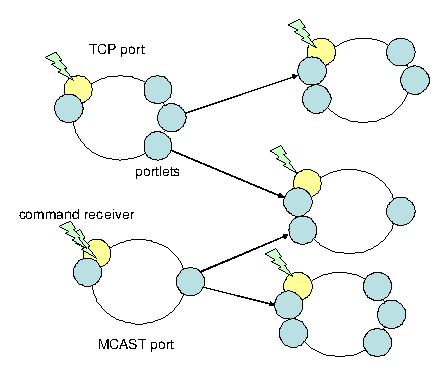
\includegraphics[width=10cm]{fig-port-portlets}
}
\caption[Interprocess communication model]{ 
%
Communications model.  Every process or thread can own
any number of ports.  Every port can be directed to send
data to any number of other ports.  Since different
processes will access this data at different rates,
it is useful to consider each port as owning several
``portlets'' that manage each individual link to another
port.  Given the most conservative quality of service settings,
data will persist in the communications system 
as long as is necessary to send it on the slowest link.
%
}
\label{fig:yarp-port}
\end{figure}

The main abstraction for inter-process communication is called a
port. A port template class can be specialized to send any data type
across an IP-network relying on a set of different
protocols. Depending on the protocol different behaviors can be
obtained the implemented protocols include TCP, UDP, MCAST, QNET1, and
shared memory. A port can either send to many target ports or receive
simultaneously from many other ports. A port is an active object: a
thread continuously services the port object. Being an active object
allows responding to external events at run time, and for example it
is possible to send commands to port objects to change their
behavior. Commands include connecting to another remote port or
receiving an incoming request for connection and since all this can be
done at run-time it naturally enables connecting/disconnecting parts
of the control system on the fly.


Figure~\ref{fig:yarp-port} shows an exemple structure of the port
abstraction. Each port is, in practice, a complex object managing many
communication channels of the same data type. Each port is potentially
both an input and output device although for simplicity of use only
one modality is actually allowed in practice. This is enforced by the
class definition and the C++ type check. Each communication channel is
managed by a portlet object within the main port. Different situations
are illustrated in Figure~\ref{fig:yarp-port}: for example an MCAST
port relies on the protocol itself to send to multiple targets while
on the contrary a TCP port has to instantiate multiple portlets to
connect to multiple targets. In cases where the code detects that two
ports are running on the same machine the IP protocol is replaced by a
shared memory connection. In Figure~\ref{fig:yarp-port} a special
portlet is shown: this is indicated as command receiver. As already
mentioned its function is that of receiving commands to connect,
disconnect, or generically operating on the port. Further ports can
run independently without blocking the calling process (if desired) or
they can wake up the calling process on the occurrence of new data. In
some cases synchronous communication is allowed (TCP protocol).

Protocols can be intermixed following certain rules. Different
operating systems can of course communicate to each other. QNET
protocol is an exception and it is only valid within a QNX network.

YARP communication code leads to a componentization of the control
architecture into many cooperating modules. The data sent through port
can range from simple integral types to complex objects such as arrays
of data (images) or vectors. Thus controlling a robot becomes
something like writing a distributed network of such modules.

In addition, YARP contains supporting libraries for mathematics and
robot type computation (kinematics, matrices, vectors, etc.), image
processing (compatible with the Intel IPL library), and general
purpose utility classes. We also designed a few modules based on
existing Microsoft technology to allow remote controlling Windows
machines (this support comes naturally on QNX). In short, these
scriptable modules complete seamlessly the architecture allowing the
design of scripts to bring up the whole control structure and connect
many modules together.

A Matlab interface to ports has been implemented. This allows building
Matlab modules (e.g. .m files) that connect to the robot to read/write
data. There are basically two advantages: i) complex algorithms can be
quickly implemented and tested relying on Matlab existing toolboxes,
ii) an additional level of scripting can be realized within
Matlab. Matlab provides a relatively efficient and easy to use display
library that can be used to visualize the functioning and performance
of an ongoing experiment.

\subsection{Robot independent code}

One of the goals in writing our control architecture has been that of
simplifying the programming of a complex robotic structure such as a
humanoid robot. Control cards come in many different flavors and
programming them is usually painful. It would be much better if a
standardized interface were provided. It would be even better if a
suitable abstraction were available.

To solve the first problem we defined a virtual device driver
interface into YARP. To solve the second, we encapsulated the control
of parts of the robot (head, arm, frame grabbers, etc.) into a
standardized template class hierarchy.

In short, the virtual device drivers bear much of their structure from
the UNIX device drivers. Each cards driver class contains three main
methods: Open, Close, and IOCtl. The latter is the core of the
interface. Each device accepts a set of messages (with parameters)
through the IOCtl call. Each message accomplishes a specific
function. Two different control cards supporting roughly the same
commands can be easily (as it was done in our setup) mapped into
exactly the same virtual device driver structure, although clearly the
implementation might differ.

The next layer is a C++ hierarchy of classes which through templates
includes both the specification of the controlling device driver
(e.g. the head is controlled through a certain control card) and the
idiosyncrasies of the particular setup (e.g. wiring of the robot might
differ, or initialization might require different calibration
procedures). 


\subsection{Robot specific interface}

The real communication with the robot is carried out through a set of
binary modules that use a device driver structure. Module
customization is at this stage accomplished through configuration
files. In the YARP language these modules are called daemons (a term
borrowed from UNIX). The daemons directly interact with the remainder
of the robot software through YARP ports and in general they export
very specialized communication channels. For example the frame grabber
has an output port of type image and the head control daemon an input
port that accepts velocity commands. There are no specific
restrictions on the type of ports exported by a daemon since any type
of state information about the modules might be required.

Further, some of the daemons accept or send commands of a special type
that are generally used to communicate status information. A bus
structure based on the MCAST protocol has been implemented to transmit
and receive these special messages (called bottles). YARP bottles may
contain any type of data or even a group of heterogeneous elements of
different types. The structure contains identifiers to properly decode
messages and interpret the data. YARP bottles create a network within
the network of behaviors to realize a high-level control and
coordinate a large number of modules.


